\section{Circuitos digitais, expressões booleanas e tabela verdade}
\frame{
	\frametitle{O que vimos até agora?}
	\begin{block}{}
		\begin{itemize}
			\item Circuitos Lógicos.
			\item Expressões booleanas.
			\item Tabela verdade.
		\end{itemize}
	\end{block}
	\centerline{\includegraphics[width=0.75\linewidth]{Figuras/Ch4/conversao04.png}}
}

\frame{
	\frametitle{Como projetar um circuito digital?}
	\centering
	\begin{tikzpicture}[node distance=0.5cm, base/.style={
		% The shape:
		rectangle,minimum height=1cm,minimum width=1.5cm,rounded corners=3mm,align=center,
		% The rest
		very thick,draw=black!50,
		fill=black!20}]
	
		\node[base] (S) {Situação};
		\node[base,right=of S,text width=1.5cm] (TV) {Tabela verdade};
		\node[base, right=of TV, text width=2cm] (ES) {Expressão simplificada};
		\node[base, right=of ES] (C) {Circuito};
		
		\graph {(S) -> (TV) -> (ES) -> (C);};
		
	\end{tikzpicture}
%	\centerline{\includegraphics[width=0.75\linewidth]{Figuras/Ch4/resumo04.png}}
}

\frame{
	\frametitle{Resolução de projetos lógicos}
%	\centerline{\includegraphics[width=0.75\linewidth]{Figuras/Ch4/2var.PNG}} 
	\begin{block}{Exemplo com duas variáveis}
		Caso tenha carro na(s)...
		\begin{itemize}
			\item Rua B
			\item Rua A
			\item Ruas A e B
		\end{itemize}
	\end{block}

	\centering
	\scalebox{0.9}{

\tikzset{every picture/.style={line width=0.75pt}} %set default line width to 0.75pt        

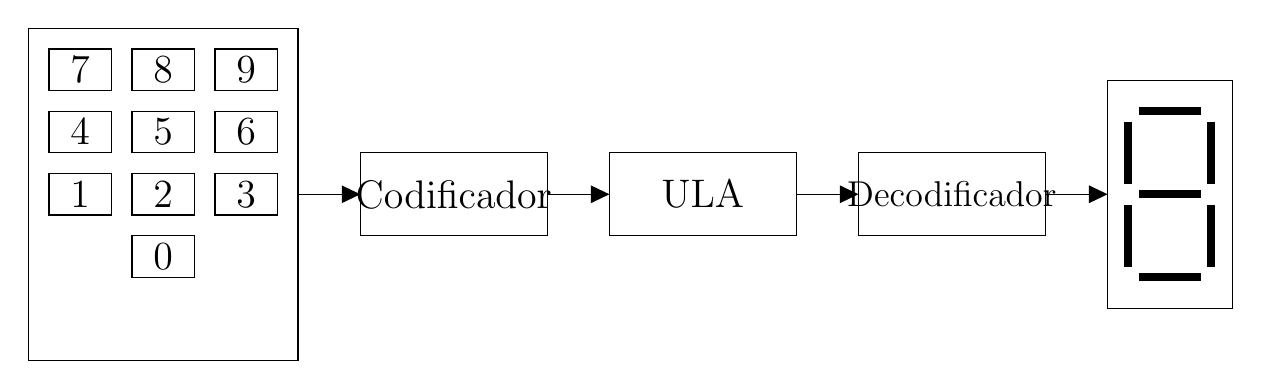
\begin{tikzpicture}[x=0.75pt,y=0.75pt,yscale=-1,xscale=1]
%uncomment if require: \path (0,300); %set diagram left start at 0, and has height of 300

%Shape: Rectangle [id:dp8798188650405219] 
\draw   (30,50) -- (160,50) -- (160,210) -- (30,210) -- cycle ;
%Shape: Rectangle [id:dp593444354888008] 
\draw   (40,60) -- (70,60) -- (70,80) -- (40,80) -- cycle ;
%Shape: Rectangle [id:dp4412846627526852] 
\draw   (80,60) -- (110,60) -- (110,80) -- (80,80) -- cycle ;
%Shape: Rectangle [id:dp2343273962035186] 
\draw   (120,60) -- (150,60) -- (150,80) -- (120,80) -- cycle ;
%Shape: Rectangle [id:dp05777918912875246] 
\draw   (40,90) -- (70,90) -- (70,110) -- (40,110) -- cycle ;
%Shape: Rectangle [id:dp9955010424516375] 
\draw   (80,90) -- (110,90) -- (110,110) -- (80,110) -- cycle ;
%Shape: Rectangle [id:dp24021539717259266] 
\draw   (120,90) -- (150,90) -- (150,110) -- (120,110) -- cycle ;
%Shape: Rectangle [id:dp36169684584711925] 
\draw   (40,120) -- (70,120) -- (70,140) -- (40,140) -- cycle ;
%Shape: Rectangle [id:dp7232437677097003] 
\draw   (80,120) -- (110,120) -- (110,140) -- (80,140) -- cycle ;
%Shape: Rectangle [id:dp6884539525496838] 
\draw   (120,120) -- (150,120) -- (150,140) -- (120,140) -- cycle ;
%Shape: Rectangle [id:dp9961423077173726] 
\draw   (80,150) -- (110,150) -- (110,170) -- (80,170) -- cycle ;
%Shape: Rectangle [id:dp6643057105712631] 
\draw   (190,110) -- (280,110) -- (280,150) -- (190,150) -- cycle ;
%Shape: Rectangle [id:dp7094011053258715] 
\draw   (550,75) -- (610,75) -- (610,185) -- (550,185) -- cycle ;
%Shape: Rectangle [id:dp2693438921699036] 
\draw   (310,110) -- (400,110) -- (400,150) -- (310,150) -- cycle ;
%Shape: Rectangle [id:dp3654960401722005] 
\draw   (430,110) -- (520,110) -- (520,150) -- (430,150) -- cycle ;
%Straight Lines [id:da6667328032348829] 
\draw    (160,130) -- (188,130) ;
\draw [shift={(190,130)}, rotate = 180] [fill={rgb, 255:red, 0; green, 0; blue, 0 }  ][line width=0.75]  [draw opacity=0] (8.93,-4.29) -- (0,0) -- (8.93,4.29) -- cycle    ;

%Straight Lines [id:da5165651690517046] 
\draw    (280,130) -- (308,130) ;
\draw [shift={(310,130)}, rotate = 180] [fill={rgb, 255:red, 0; green, 0; blue, 0 }  ][line width=0.75]  [draw opacity=0] (8.93,-4.29) -- (0,0) -- (8.93,4.29) -- cycle    ;

%Straight Lines [id:da17751850693095572] 
\draw    (400,130) -- (428,130) ;
\draw [shift={(430,130)}, rotate = 180] [fill={rgb, 255:red, 0; green, 0; blue, 0 }  ][line width=0.75]  [draw opacity=0] (8.93,-4.29) -- (0,0) -- (8.93,4.29) -- cycle    ;

%Straight Lines [id:da4998570413390182] 
\draw [color={rgb, 255:red, 0; green, 0; blue, 0 }  ,draw opacity=1 ][line width=3]    (560,95) -- (560,125) ;


%Straight Lines [id:da05287212083080073] 
\draw [color={rgb, 255:red, 0; green, 0; blue, 0 }  ,draw opacity=1 ][line width=3]    (600,95) -- (600,125) ;


%Straight Lines [id:da9146969001147236] 
\draw [color={rgb, 255:red, 0; green, 0; blue, 0 }  ,draw opacity=1 ][line width=3]    (560,135) -- (560,165) ;


%Straight Lines [id:da37610179690179124] 
\draw [color={rgb, 255:red, 0; green, 0; blue, 0 }  ,draw opacity=1 ][line width=3]    (600,135) -- (600,165) ;


%Straight Lines [id:da2798262228013664] 
\draw [color={rgb, 255:red, 0; green, 0; blue, 0 }  ,draw opacity=1 ][line width=3]    (595,130) -- (565,130) ;


%Straight Lines [id:da15184615547446478] 
\draw [color={rgb, 255:red, 0; green, 0; blue, 0 }  ,draw opacity=1 ][line width=3]    (595,90) -- (565,90) ;


%Straight Lines [id:da20609816632014244] 
\draw [color={rgb, 255:red, 0; green, 0; blue, 0 }  ,draw opacity=1 ][line width=3]    (595,170) -- (565,170) ;


%Straight Lines [id:da16937059284664002] 
\draw    (520,130) -- (548,130) ;
\draw [shift={(550,130)}, rotate = 180] [fill={rgb, 255:red, 0; green, 0; blue, 0 }  ][line width=0.75]  [draw opacity=0] (8.93,-4.29) -- (0,0) -- (8.93,4.29) -- cycle    ;


% Text Node
\draw (135,70) node   {\Large $9$};
% Text Node
\draw (95,70) node   {\Large $8$};
% Text Node
\draw (55,70) node   {\Large $7$};
% Text Node
\draw (135,100) node   {\Large $6$};
% Text Node
\draw (135,130) node   {\Large $3$};
% Text Node
\draw (95,160) node   {\Large $0$};
% Text Node
\draw (95,130) node   {\Large $2$};
% Text Node
\draw (95,100) node   {\Large $5$};
% Text Node
\draw (55,100) node   {\Large $4$};
% Text Node
\draw (55,130) node   {\Large $1$};
% Text Node
\draw (235,130) node  [align=left] {\Large Codificador};
% Text Node
\draw (355,130) node  [align=left] {\Large ULA};
% Text Node
\draw (475,130) node [scale=0.9] [align=left] {\Large Decodificador};


\end{tikzpicture}
}
}

\frame{
	\frametitle{Resolução de projetos lógicos}
	
	\begin{block}{Exemplo com três variáveis}
		Conexão de 3 aparelhos a um amplificador, obedecendo às prioridades:
		\begin{itemize}
			\item CD player
			\item Tape playback
			\item Radio receptor
		\end{itemize}
	\end{block}

	\bigskip

	\centerline{\includegraphics[width=1\linewidth]{Figuras/Ch4/3var.PNG}} 
}

\frame{
	\frametitle{Resolução de projetos lógicos}
	\begin{block}{Exemplo com quatro variáveis}
		Conexão de 4 setores, via intercomunicadores, a central da Secretária, obedecendo às prioridades:
		\begin{itemize}
			\item Presidente
			\item Vice Presidente
			\item Engenharia
			\item Chefes de Seção
		\end{itemize}
	\end{block}

	\centerline{\includegraphics[width=1\linewidth]{Figuras/Ch4/4var.PNG}} 
}


\frame{
	\frametitle{Obtendo a expressão a partir do circuito - Exemplo \#01}
	\begin{center} \begin{circuitikz} \draw
			(0,2) node[and port] (myand) {}
			(2,1) node[or port] (myor) {}
			(myand.in 1) node[left=.5cm](a) {A}
			(myand.in 2) node[left =.5cm](b) {B}
			(myand.out) -| (myor.in 1)
			(a) -| (myand.in 1)
			(b) -| (myand.in 2)
			(b) node[below=1cm](c){C}
			(c) -| (myor.in 2)
			(myor.out) -- ++(.5cm,0) node[right] {S};
		\end{circuitikz} \end{center}
}

\frame{
	\frametitle{Obtendo a expressão a partir do circuito - Exemplo \#02}
	\begin{center} \begin{circuitikz}
			\draw
			(0,2) node[or port] (myor) {}
			(0,0) node[not port, scale=.5] (mynot) {}
			(2,1) node[nand port] (mynand) {}
			(myor.in 1) node[left=0.5cm](a) {A}
			(myor.in 2) node[left =.5cm](b) {B}
			(myor.out) -| (mynand.in 1)
			(a) -| (myor.in 1)
			(b) -| (myor.in 2);
			\node[coordinate] (p1) at ($ (myor.in 1)+(-0.5cm,0) $) {};
			\node[] (c) at (p1 |- mynot.in) {};
			\draw (mynot.in) -- (c) node[left] {C}
			(mynot.out) -| (mynand.in 2)
			(mynand.out) -- ++(.5cm,0) node[right] {S};
		\end{circuitikz} \end{center}
}

\frame{
	\frametitle{Obtendo a expressão a partir do circuito - Exemplo \#03}
	\begin{center} \begin{circuitikz} \draw
			(0,4) node[nor port] (mynor) {}
			(0,2) node[and port] (myand) {}
			(0,0) node[not port, scale=.5] (mynot) {}
			(2,3) node[nand port] (mynand) {}
			(4,1) node[or port] (myor) {}
			(mynor.in 1) node[left=.5cm](a) {A}
			(mynor.in 2) node[left =.5cm](b) {B}
			(mynor.out) -| (mynand.in 1)
			(myand.in 1) node[left=.5cm](c) {C}
			(myand.in 2) node[left =.5cm](d) {D}
			(myand.out) -| (mynand.in 2);
			\node[coordinate] (p1) at ($ (mynor.in 1)+(-0.5cm,0) $) {};
			\node[] (e) at (p1 |- mynot.in) {};
			\draw (a) -| (mynor.in 1)
			(b) -| (mynor.in 2)
			(c) -| (myand.in 1)
			(d) -| (myand.in 2)
			(mynot.in) -- (e) node[left] {E}
			(mynand.out) -| (myor.in 1)
			(mynot.out) -| (myor.in 2)
			(myor.out) -- ++(.5cm,0) node[right] {S};
		\end{circuitikz} \end{center}
}


\frame{
	\frametitle{Obtendo o circuito a partir da expressão}
	\begin{block}{Hierarquia}
		\begin{itemize}
			\item Parênteses.
			\item Bloco AND.
			\item Bloco OR.
			\item Negação.
		\end{itemize}
	\end{block}
}

\frame{
	\frametitle{Obtendo o circuito a partir da expressão}
	\begin{block}{Exercícios}
		\begin{itemize}
			\item $S = (A + B)\cdot C\cdot (B+D)$
			\item $Z = (\notted{A\cdot B} \oplus A) + (\notted{A} + B)$
			\item $Y = (A\cdot B) + \notted{C}\cdot D$
			\item $X = (A + B + C)\cdot \notted{(\notted{A} + C)\cdot (A + \notted{B})}$
		\end{itemize}
	\end{block}
}

\frame{
	\frametitle{Obtendo a tabela verdade a partir da expressão}
	\begin{block}{Tabela verdade}
		A \textbf{tabela verdade} deve registrar \textbf{todas as possibilidades} de um dada expressão booleana, e pode ser obtida através dos seguintes passos:
		\begin{enumerate}
			\item Monte o quadro de possibilidades.
			\item \textbf{n} colunas para as variáveis.
			\item Use colunas auxiliares para os membros.
			\item Monte uma coluna para o resultado final.
		\end{enumerate}
	\end{block}
}

\frame{
	\frametitle{Obtendo a tabela verdade a partir da expressão}
	\begin{block}{Exemplo \#01}
		\[ Z = (\notted{A\cdot B} \oplus A) + (\notted{A} + B) \]
		
		\bigskip
		\centering
%		\renewcommand{\arraystretch}{1}
		\resizebox{1\textwidth}{!}{
		\begin{tabular}{cc|c|c|c|c|c}
			\toprule
			$ A $ & $ B $ & $\notted{A\cdot B} $ & $\notted{A\cdot B} \oplus A$ & $\notted{A}$ & $\notted{A} + B$ & \textcolor{green}{S} \\ \midrule
			0 & 0 & 1 &	\textcolor{red}1 & 1 & \textcolor{red}1 & \textcolor{blue}1 \\
			0 & 1 & 1 & \textcolor{red}1 & 1 & \textcolor{red}1 & \textcolor{blue}1 \\
			1 & 0 & 1 & \textcolor{red}0 & 0 & \textcolor{red}0 & \textcolor{blue}0 \\
			1 & 1 & 0 & \textcolor{red}1 & 0 & \textcolor{red}1 & \textcolor{blue}1 \\  \bottomrule
	\end{tabular}}
	\end{block}
}

\frame{
	\frametitle{Obtendo a tabela verdade a partir da expressão}
	\begin{block}{Exercícios}
		\begin{itemize}
			\item $S = (A\cdot \notted{B}\cdot C) + (A\cdot \notted{D}) + (\notted{A}\cdot B\cdot D)$
			\item $Z = \notted{A} + B + A\cdot \notted{B}\cdot \notted{C}$
			\item $Y = C \oplus (\notted{A.B})$
			\item $X = A\cdot \notted{B} + \notted{A}\cdot B$
		\end{itemize}
	\end{block}
}

\frame{
	\frametitle{Obtendo a expressão a partir da tabela verdade}
	\begin{block}{Situação mais utilizada}
		\textbf{Lembre-se do problema inicial}
		\begin{itemize}
			\item Situação.
			\item Tabela verdade.
			\item Expressão booleana.
			\item Circuito lógico.
		\end{itemize}
			
			\bigskip
			
			\textbf{MINTERMOS}: saídas iguais a \textbf{1} - \textcolor{red}{SoP}
			
			\bigskip
			
			\textbf{MAXTERMOS}: saídas iguais a \textbf{0} - \textcolor{red}{PoS}
	\end{block}
}

\frame{
	\frametitle{Obtendo a expressão a partir da tabela verdade}
	\begin{block}{MINTERMOS}
		\begin{itemize}
			\item Saídas iguais a \textbf{1} - \textcolor{red}{SoP}
		\end{itemize}
	\end{block}

	\renewcommand{\arraystretch}{1}
	\centering
	\begin{tabular}{ccc|c}
		\toprule
		A & B & C & S                \\ \midrule
		0 & 0 & 0 & \textcolor{red}1 \\
		0 & 0 & 1 & \textcolor{red}1 \\
		0 & 1 & 0 & \textcolor{red}1 \\
		0 & 1 & 1 & 0                \\
		1 & 0 & 0 & 0                \\
		1 & 0 & 1 & \textcolor{red}1 \\
		1 & 1 & 0 & 0                \\
		1 & 1 & 1 & \textcolor{red}1 \\ \bottomrule
	\end{tabular}

	\begin{block}{Expressão final}
		\vspace{-0.3cm}
		\[ S = (\notted{A} \cdot \notted{B}\cdot \notted{C}) + (\notted{A} \cdot \notted{B}\cdot C) + (\notted{A}\cdot B\cdot \notted{C}) + (A\cdot \notted{B}\cdot C) + (A\cdot B\cdot C) \]
	\end{block}

}

\frame{
	\frametitle{Obtendo a expressão a partir da tabela verdade}
	\begin{block}{MAXTERMOS}
		\begin{itemize}
			\item Saídas iguais a \textbf{0} - \textcolor{red}{PoS}
		\end{itemize}
	\end{block}

	\renewcommand{\arraystretch}{1}
	\centering
	\begin{tabular}{ccc|c}
		\toprule
		A & B & C & S                        \\ \midrule
		0 & 0 & 0 & 1                        \\
		0 & 0 & 1 & 1                        \\
		0 & 1 & 0 & 1                        \\
		0 & 1 & 1 & \textcolor{red}0         \\
		1 & 0 & 0 & \textcolor{red}0         \\
		1 & 0 & 1 & 1                        \\
		1 & 1 & 0 & \textcolor{red} 0        \\ 
		1 & 1 & 1 & 1                        \\ \bottomrule
	\end{tabular}

	\begin{block}{Expressão final}
		\vspace{-0.15cm}
		\[ S = (A + \notted{B} + \notted{C})\cdot (\notted{A}  + B + C)\cdot (\notted{A} + \notted{B} + C) \]
	\end{block}
}


\section*{Exercícios}
\frame{
	\frametitle{Exercícios}
	\begin{block}{}
		01. A partir da tabela verdade abaixo encontre a expressão booleana por mintermos e maxtermos. Após isto, implemente ambos os circuitos digitais.
	\end{block}

	\medskip

	\renewcommand{\arraystretch}{1}
	\centering
	\begin{tabular}{ccc|c}
		\toprule
		A & B & C & S \\ \midrule
		0 & 0 & 0 & 0 \\
		0 & 0 & 1 & 1 \\
		0 & 1 & 0 & 1 \\
		0 & 1 & 1 & 0 \\
		1 & 0 & 0 & 1 \\
		1 & 0 & 1 & 0 \\
		1 & 1 & 0 & 0 \\
		1 & 1 & 1 & 1 \\ \bottomrule
	\end{tabular}
}

\section*{Referências}


\frame{
	\frametitle{Referências e exercícios complementares}
	\begin{itemize}
		\item IDOETA, Ivan V. e CAPUANO, Francisco G. Elementos de Eletrônica Digital. São Paulo:
		      Editora Érica, ed. 40. 2008.
	\end{itemize}

	\centering{\alert{Página 82 - \textbf{2.9.2 até 2.9.13, 2.9.15 até 2.9.17}}}

}